%% IEEE AIoT 2026: Conference Paper Submission
%% DOUBLE-BLIND SUBMISSION
%% Template: IEEE Conference Template (June 2024 revision)
%% Track:    Track 3: Edge, Cloud, and Fog Computing in IoT
%%
%% =====================================================================
%% HARD PAGE LIMIT: 6 pages TOTAL including references.
%% This manuscript MUST NOT exceed 6 pages under any circumstances.
%% IEEE AIoT 2026 camera-ready limit.
%% =====================================================================
%%
\documentclass[conference]{IEEEtran}
\IEEEoverridecommandlockouts
\usepackage{cite}
\usepackage{amsmath,amssymb,amsfonts}
\usepackage{algorithmic}
\usepackage{graphicx}
\usepackage{textcomp}
\usepackage{xcolor}
\usepackage{booktabs}
\usepackage{multirow}
\usepackage{array}
\usepackage{url}
\usepackage{flushend}
\usepackage{pgfplots}
\usepgfplotslibrary{groupplots}
\pgfplotsset{compat=1.17}
\def\BibTeX{{\rm B\kern-.05em{\sc i\kern-.025em b}\kern-.08em
T\kern-.1667em\lower.7ex\hbox{E}\kern-.125emX}}
\begin{document}
\title{Curate for Attention, Sample for Convolutions: Taming False Alarms in Continuous Edge AIoT Sensing}
\author{\IEEEauthorblockN{Anonymous Authors}
\IEEEauthorblockA{Institution redacted for double-blind review}}
\maketitle
\begin{abstract}
Deep learning detectors deployed in continuous edge Artificial Intelligence of
Things (AIoT) sensing encounter severe temporal class imbalance: over 80\% of
operational frames contain no targets. While training with negative (background-only)
frames suppresses false alarms, existing studies optimize negative ratios for single
architectures in isolation, leaving open whether curation rules transfer across
paradigms. We present a cross-architecture empirical study across four matched-capacity
($2.3$--$2.6$\,M parameters) lightweight edge detectors (YOLO11n, YOLO26n, YOLO12n,
and YOLOv10n) spanning convolutional, hybrid, attention-centric, and dual-assignment
designs. Sweeping five nested ratio configurations (0\%--80\% negatives) on a
15,723-frame driver-monitoring corpus, we find that while false-alarm suppression
trajectories diverge by up to 31.5$\times$, all four architectures converge to a
narrow operational false-alarm band ($3.14$--$7.08\,\mathrm{FP/1k}$) at 80\% negatives.
Our results demonstrate that negative-frame prevalence, rather than architectural bias
or inference latency, governs operational reliability in continuous edge AIoT sensing.
\end{abstract}
\begin{IEEEkeywords}
Artificial Intelligence of Things (AIoT), edge intelligence, driver monitoring
systems (DMS), object detection, negative frames, hard-negative mining, class imbalance,
false-positive rate, You Only Look Once (YOLO), area attention.
\end{IEEEkeywords}
\section{Introduction}
\label{sec:intro}

Vision systems deployed in continuous edge Artificial Intelligence of Things (AIoT)
sensing operate under extreme temporal class imbalance~\cite{b1}. In vehicular
driver monitoring systems (DMS), cameras continuously process video across multi-hour
trips, yet safety-critical cues (e.g., mobile phone usage, drinking, yawning)
occupy a small fraction of the operational stream~\cite{b12}, with over 80\% of
frames containing no targets.

Consequently, an edge detector's operational viability is governed not merely by
mean average precision ($\mathrm{mAP}$) on dense benchmarks, but primarily by its
ability to maintain silence on background frames. Non-trivial false-alarm rates induce
nuisance alerts that exhaust battery and thermal envelopes, consume cellular quotas,
and precipitate driver alert fatigue~\cite{b12,b13}.

Injecting background-only frames during training mitigates false alarms. Practitioner
heuristics advise 0--10\% background imagery~\cite{b8}, while domain literature
shows that omitting negatives degrades open-world reliability~\cite{b5,b6}. However,
prior studies evaluate single architectures in isolation. It remains unproven whether
optimal negative ratios or curation policies transfer across feature-aggregation
mechanisms. If negative sensitivity is architecture-dependent, detector selection and
dataset curation must be jointly co-designed.

We evaluate four matched-capacity ($2.3$--$2.6\text{M}$ parameter) detectors from the
You Only Look Once (YOLO) family: YOLO11n~\cite{b9}, YOLO26n~\cite{b10},
YOLO12n~\cite{b11}, and YOLOv10n~\cite{b20}, spanning hybrid conv-attention, pure
convolution, area-attention, and dual-assignment NMS-free paradigms. On a 15,723-frame
corpus with 80.9\% natural negative dominance, we investigate two research questions:
\begin{itemize}
\item \textbf{RQ1 (Ratio Sensitivity):} How does negative-frame scaling affect
false-alarm suppression across architectures, and does the ratio optimizing
detection accuracy differ between paradigms?
\item \textbf{RQ2 (Curation Quality):} At a reference ratio ($r_{\mathrm{ref}} = 40\%$),
does substituting random negatives with hard-mined negatives yield further
suppression at matched dataset cardinality?
\end{itemize}

Our contributions are threefold: (1)~the first cross-architecture negative-ratio sweep
across four matched-capacity edge detectors on a safety-critical AIoT dataset; (2)~a
controlled hard-negative mining benchmark at matched cardinality ($r_{\mathrm{ref}}{=}40\%$),
isolating sample entropy from volume; (3)~an empirical latency benchmark ($7.7$--$21.7$\,ms)
coupled with an analytical translation from $\mathrm{FP/1k}$ to hourly nuisance alerts
($\mathcal{A}_h$), demonstrating that data curation governs edge reliability independently
of inference latency.

\section{Related Work}
\label{sec:related}

\textbf{Class Imbalance and Negative Sampling.}
Foreground-background imbalance in object detection has traditionally been mitigated
via loss reweighting~\cite{b1}, online hard-region mining~\cite{b14,b4}, dynamic
sample assignment~\cite{b3}, and representation drift tracking~\cite{b2}. However,
these techniques operate on candidate proposals \textit{within positive, object-containing images}.
In continuous edge AIoT sensing, the predominant operational failure mode is
inter-frame: entire video frames contain zero targets, yet provoke spurious detections
that waste edge compute cycles, trigger unnecessary cellular transmissions, and induce
operator alert fatigue~\cite{b12,b13}.

\textbf{Lightweight Edge Detectors.}
Edge AIoT deployments mandate compact architectures capable of real-time inference
under strict compute and thermal envelopes~\cite{b15}. Modern edge detectors reflect
fundamentally distinct feature-aggregation and assignment paradigms: hybrid
convolutional-attention models like YOLO11~\cite{b9} incorporate neck self-attention
(C2PSA); pure convolutional networks like YOLO26~\cite{b10} leverage structural
reparameterization (RepConv) for efficient feedforward processing; attention-centric
models like YOLO12~\cite{b11} employ Area Attention (A2C2f) to retain global receptive
fields with linear complexity; and dual-assignment models like YOLOv10~\cite{b20}
eliminate post-processing NMS via consistent one-to-one heads.
Evaluating these architectures at strictly matched capacity ($2.3$--$2.6\text{M}$
parameters) isolates the impact of spatial aggregation and assignment mechanics on
background suppression.

\textbf{Negative-Frame Training in AIoT.}
While practitioner guidelines advise injecting 0--10\% background frames~\cite{b8},
empirical studies in camera-trap ecology~\cite{b5} and autonomous driving~\cite{b6}
demonstrate that omitting background images severely degrades open-world false-alarm
resilience. In human-object interaction, scaling negative pairs up to 1000:1 is
essential to regularize complex spatial relationships~\cite{b7}. In vehicular DMS~\cite{b12,b17}, standard datasets~\cite{b18,b19} prioritize
positive cue diversity, but deployed systems encounter vast stretches of routine,
unannotated driving. Crucially, prior investigations optimize negative ratios for a
single architecture in isolation; no prior work examines whether optimal negative-frame
prevalence or hard-negative curation transfers across architectural paradigms.

\section{Methodology}
\label{sec:methodology}

\subsection{Problem Formulation}
\label{subsec:formulation}
In continuous edge AIoT video streams $\mathcal{S} = \{X_t\}_{t=1}^T$, frames are partitioned into positive ($\mathcal{D}_{\mathrm{pos}}$, containing driver safety cues) and background-only frames ($\mathcal{D}_{\mathrm{neg}}$, devoid of targets). For a detector $f_\theta$, predicted bounding boxes filtered at operational confidence threshold $\tau \in (0, 1]$ yield the detection set $\hat{\mathcal{Y}}_\tau(X)$. Because negative frames contain no ground truth ($Y = \emptyset$), any detection in $\hat{\mathcal{Y}}_\tau(X)$ represents an operational false alarm.

We evaluate deployment reliability via two metrics on the held-out negative test set $\mathcal{D}_{\mathrm{test}}^{\mathrm{neg}}$ ($1{,}272$ frames):
\begin{equation}
\mathrm{FP/1k} = \frac{1000}{|\mathcal{D}_{\mathrm{test}}^{\mathrm{neg}}|} \sum_{X \in \mathcal{D}_{\mathrm{test}}^{\mathrm{neg}}} |\hat{\mathcal{Y}}_\tau(X)|,
\label{eq:fp1k}
\end{equation}
and the projected hourly nuisance alert rate $\mathcal{A}_h$ at camera frame rate $f_{\mathrm{FPS}}$ (in frames per second, FPS):
\begin{equation}
\mathcal{A}_h = 3.6 \, f_{\mathrm{FPS}} \, p_{\mathrm{neg}} \, \mathrm{FP/1k},
\label{eq:nuisance}
\end{equation}
where $p_{\mathrm{neg}} \in (0, 1]$ is the natural operational negative prevalence ($p_{\mathrm{neg}} \approx 0.809$ in our vehicular corpus). Operational false alarms ($\mathrm{FP/1k}$ and $\mathcal{A}_h$) are measured at operational threshold $\tau = 0.25$ and NMS intersection over union ($\mathrm{IoU} = 0.70$). Standard detection accuracy metrics ($\mathrm{mAP}_{50}$, $\mathrm{mAP}_{50:95}$, precision $\mathrm{P}$, recall $\mathrm{R}$) are evaluated across the full confidence spectrum, with $\mathrm{P}$ and $\mathrm{R}$ reported at the maximum-$F_1$ operating point.

\subsection{Architectural Loss Dynamics on Negative Frames}
\label{subsec:loss_mechanics}
All four evaluated detectors utilize dense anchor-free feature pyramids. On unannotated background frames ($Y{=}\emptyset$), positive anchor assignment yields zero matches across all pyramid scales. Consequently, bounding-box regression loss ($\mathcal{L}_{\mathrm{box}}$) and distribution focal loss ($\mathcal{L}_{\mathrm{dfl}}$) vanish identically, collapsing the total supervisory signal strictly to classification binary cross-entropy (BCE) over all spatial grid cells:
\begin{equation}
\mathcal{L}_{\mathrm{det}}^{\mathrm{neg}} = -\lambda_{\mathrm{cls}} \sum_{s=1}^S \sum_{i=1}^{H_s W_s} \sum_{c=1}^C \log\left(1 - \hat{p}_{s, i, c}\right).
\label{eq:det_neg_loss}
\end{equation}
Although this loss formulation is mathematically shared, how negative gradients propagate back through the network depends fundamentally on architectural feature aggregation:
\begin{itemize}
\item \textbf{Pure Reparameterized Convolution (YOLO26n):} Gradients update strictly localized convolutional neural network (CNN) filters (RepConv), penalizing spatial kernels that fire on high-frequency edges resembling driver cues (e.g., steering wheel arcs, seatbelt fixtures).
\item \textbf{Hybrid Attention (YOLO11n):} Gradients update both convolutional backbones and neck-level partial self-attention projections (C2PSA), modulating prominent spatial feature locations across wider contexts.
\item \textbf{Linear Area Attention (YOLO12n):} Gradients propagate through Area Attention modules (A2C2f) partitioned across horizontal and vertical visual areas, enabling dynamic receptive fields that suppress extended structural patterns (e.g., window reflections, headrest contours).
\item \textbf{Dual-Assignment Head (YOLOv10n):} Gradients simultaneously supervise auxiliary one-to-many and primary one-to-one heads, enforcing background silence without relying on post-processing NMS heuristics.
\end{itemize}
This structural divergence underpins our investigation into whether negative-frame configurations transfer across detection paradigms.

\subsection{Dataset and Partitioning}
\label{subsec:dataset}
Experiments utilize a 15,723-frame in-cabin DMS corpus captured under diverse lighting, driver subjects, vehicle interiors, and viewpoints with institutional consent and de-identification. The dataset contains 3,001 positive frames annotated with verified two-dimensional (2D) bounding boxes across four driver-cue categories: \texttt{phone\_use} (2,437 frames, 81.2\%), \texttt{drinking} (264 frames, 8.8\%), \texttt{yawning} (159 frames, 5.3\%), and \texttt{hand\_over\_mouth} (141 frames, 4.7\%). The remaining 12,722 frames contain no target cues, representing an 80.9\% natural negative prevalence.

A stratified 80/10/10 split ($\text{seed}{=}42$) partitions the corpus into: (1) a held-out test set of 1,572 frames (300 pos, 1,272 neg); (2) a held-out validation set of 1,572 frames (300 pos, 1,272 neg); and (3) a training universe comprising 2,401 positive frames and 10,178 candidate negatives. Both validation and test benchmarks preserve natural negative dominance (80.9\%) and remain fixed across all experiments to ensure realistic evaluation of false alarms.

\subsection{Detector Architectures}
\label{subsec:architectures}
We benchmark four lightweight nano-scale edge detectors matching micro-edge compute constraints: YOLO11n~\cite{b9}, YOLO26n~\cite{b10}, YOLO12n~\cite{b11}, and YOLOv10n~\cite{b20}. As detailed in Table~\ref{tab:architectures}, all models share matched lightweight capacity ($2.3$--$2.6\text{M}$ parameters, $6.2$--$7.6$ giga floating-point operations (GFLOPs), and latency under $22$\,ms on an NVIDIA RTX 4060 Laptop graphics processing unit (GPU)), ensuring that comparative differences reflect architectural feature aggregation rather than parameter volume.

\begin{table}[t]
\caption{Evaluated Detector Architectures (640\,$\times$\,640 Input)}
\label{tab:architectures}
\centering
\setlength{\tabcolsep}{1.6pt}
\begin{tabular}{lcccccc}
\toprule
\textbf{Model} & \textbf{Params} & \textbf{FLOPs} & \textbf{Latency$^*$} & \textbf{FPS$^*$} & \textbf{Paradigm} & \textbf{Mechanism} \\
\midrule
YOLO11n  & 2.6\,M & 6.5\,G & 16.8\,ms & 59.6 & Hybrid    & C3k2 + C2PSA \\
YOLO26n  & 2.6\,M & 6.2\,G & 21.7\,ms & 46.1 & Pure Conv & RepConv \\
YOLO12n  & 2.6\,M & 7.6\,G & 21.3\,ms & 47.0 & Attn      & A2C2f Area \\
YOLOv10n & 2.3\,M & 6.6\,G & 7.7\,ms  & 129.2 & NMS-Free & Dual-Label Head \\
\bottomrule
\end{tabular}
\vspace{1pt}
{\footnotesize $^*$Latency and throughput measured on NVIDIA RTX 4060 Laptop GPU (PyTorch, batch=1, 640\,$\times$\,640, averaged over 200 iterations after 50 warmups).}
\end{table}

\subsection{Experimental Configurations}
\label{subsec:configurations}

\subsubsection{Axis 1 (RQ1): Negative-Frame Ratio Sweep}
Holding the positive core fixed at $|\mathcal{D}_{\mathrm{pos}}| = 2{,}401$ frames, we construct five nested training subsets at uniform 20\% arithmetic increments: 0\% (2,401 total; 0 neg), 20\% (3,001 total; 600 neg), 40\% (4,001 total; 1,600 neg), 60\% (6,003 total; 3,602 neg), and 80\% (12,005 total; 9,604 neg; 574 pool negatives excluded to preserve exact 20-point stepping). Subsets are strictly nested: $\mathcal{D}_{\mathrm{neg}}^{(0\%)} \subset \mathcal{D}_{\mathrm{neg}}^{(20\%)} \subset \cdots \subset \mathcal{D}_{\mathrm{neg}}^{(80\%)}$ ($\text{seed}{=}42$). Across 4 architectures and 5 ratios, Axis~1 encompasses 20 training runs.

\subsubsection{Axis 2 (RQ2): Hard-Negative Curation}
For each architecture, a positive-only baseline ($r{=}0\%$) runs inference over the 10,178 training negatives at $\tau{=}0.25$. Mined false alarms are ranked by maximum confidence $s_{\max}(X)$, and the top $N_{\mathrm{target}}{=}1{,}600$ frames form the curated set (backfilled deterministically from remaining negatives if needed). We evaluate curation at the compute-efficient reference ratio $r_{\mathrm{ref}}{=}40\%$ with strictly matched cardinality: $|\mathcal{D}_{\mathrm{train,hard}}^{(40\%)}| = |\mathcal{D}_{\mathrm{train,rand}}^{(40\%)}| = 4{,}001\,\text{frames}$, isolating sample information entropy from volume. Axis~2 adds 8 runs (28 runs total for the primary benchmark).

\subsection{Training Protocol}
\label{subsec:protocol}
All models are fine-tuned from Common Objects in Context (COCO)-pretrained checkpoints at $640 \times 640$
resolution in single precision (FP32) using the AdamW optimizer ($\mathrm{lr}_0 = 0.00125$,
weight decay $0.0005$, batch size 16) for 100 epochs, with mosaic augmentation
disabled for the final 10 epochs (\texttt{close\_mosaic=10}). Table~\ref{tab:training}
summarizes the frozen training configuration, which is held invariant across all
detectors and ratio splits to ensure rigorous comparative isolation of feature
aggregation mechanisms. Inference latency is profiled on an NVIDIA RTX 4060
Laptop GPU, while target deployment represents embedded SoCs such as the NVIDIA
Jetson Orin Nano.

\begin{table}[t]
\caption{Unified Frozen Training Hyperparameters}
\label{tab:training}
\centering
\setlength{\tabcolsep}{5pt}
\begin{tabular}{lc}
\toprule
\textbf{Hyperparameter} & \textbf{Frozen Configuration} \\
\midrule
Input Resolution & 640\,$\times$\,640 (FP32 precision) \\
Physical / Effective Batch & 16 / 16 (no gradient accumulation) \\
Training Duration & 100 epochs \\
Optimizer & AdamW ($\mathrm{lr}_0{=}0.00125$) \\
Weight Decay & 0.0005 \\
Augmentation Cooldown & Final 10 epochs (\texttt{close\_mosaic=10}) \\
Random Seed & Fixed ($\text{seed}{=}42$) \\
\bottomrule
\end{tabular}
\vspace{1pt}
{\footnotesize Parity across models isolates feature aggregation design.}
\end{table}

\section{Experimental Results}
\label{sec:results}

\subsection{Negative-Frame Ratio Sensitivity (RQ1)}
\label{subsec:rq1_results}
Table~\ref{tab:rq1} reports detection accuracy and deployment cost across all
ratio-sweep configurations on the held-out test set (1,572 frames, 80.9\%
negative prevalence).

\begin{table}[t]
\caption{Negative-Frame Ratio Sweep across Architectures (RQ1)}
\label{tab:rq1}
\centering
\setlength{\tabcolsep}{1.2pt}
\begin{tabular}{llccccc}
\toprule
\textbf{Det.} & \textbf{$r$} & \textbf{$\mathrm{mAP}_{50}$} &
\textbf{$\mathrm{mAP}_{50\text{-}95}$} & \textbf{$\mathrm{P}$} & \textbf{$\mathrm{R}$} &
\textbf{$\mathrm{FP/1k}$} \\
\midrule
\multirow{5}{*}{YOLO11n}
& 0\%  & 0.9769 & 0.7538 & 0.8806 & 0.9741 & 59.75 \\
& 20\% & 0.9878 & 0.7518 & 0.9202 & 0.9728 & 31.45 \\
& 40\% & 0.9932 & 0.7699 & 0.9376 & 0.9839 & 24.37 \\
& 60\% & 0.9881 & \textbf{0.7747} & 0.9248 & \textbf{0.9920} & 12.58 \\
& 80\% & 0.9933 & 0.7606 & \textbf{0.9644} & 0.9766 & \textbf{4.72} \\
\midrule
\multirow{5}{*}{YOLO26n}
& 0\%  & 0.9176 & 0.7095 & 0.8649 & 0.8988 & 99.06 \\
& 20\% & 0.9744 & 0.7632 & 0.9390 & 0.9785 & 15.72 \\
& 40\% & \textbf{0.9830} & 0.7555 & 0.9411 & 0.9653 & 5.50 \\
& 60\% & 0.9660 & 0.7594 & \textbf{0.9587} & 0.9086 & 10.22 \\
& 80\% & 0.9736 & \textbf{0.7671} & 0.9217 & \textbf{0.9794} & \textbf{3.14} \\
\midrule
\multirow{5}{*}{YOLO12n}
& 0\%  & 0.9899 & 0.7653 & 0.9096 & 0.9840 & 51.89 \\
& 20\% & 0.9830 & 0.7481 & 0.9147 & 0.9837 & 35.38 \\
& 40\% & 0.9882 & \textbf{0.7772} & 0.9150 & 0.9959 & 18.08 \\
& 60\% & 0.9888 & 0.7766 & 0.9348 & \textbf{0.9960} & 9.43 \\
& 80\% & \textbf{0.9925} & 0.7529 & \textbf{0.9621} & 0.9767 & \textbf{7.08} \\
\midrule
\multirow{5}{*}{YOLOv10n}
& 0\%  & 0.9196 & 0.7124 & 0.9016 & 0.8361 & 68.40 \\
& 20\% & 0.9459 & 0.7253 & \textbf{0.9264} & 0.9083 & 23.58 \\
& 40\% & 0.9615 & 0.7428 & 0.8918 & \textbf{0.9765} & 14.15 \\
& 60\% & \textbf{0.9749} & \textbf{0.7525} & 0.9221 & 0.9758 & \textbf{4.72} \\
& 80\% & 0.9524 & 0.7384 & 0.9010 & 0.9024 & \textbf{4.72} \\
\midrule
\multicolumn{7}{l}{\textit{Cross-Model Metric Correlation with Negative Ratio ($X{=}r$, $N{=}20$)}} \\
\midrule
\multicolumn{2}{l}{Spearman $\rho$} & \multicolumn{2}{c}{---} & \textbf{+0.540}$^{*}$ & +0.227$^{\text{n.s.}}$ & \textbf{-0.921}$^{***}$ \\
\multicolumn{2}{l}{Pearson $r$}   & \multicolumn{2}{c}{---} & \textbf{+0.593}$^{*}$ & +0.264$^{\text{n.s.}}$ & \textbf{-0.824}$^{***}$ \\
\bottomrule
\end{tabular}
\vspace{1pt}
{\footnotesize Single seed ($\text{seed}{=}42$); 1,272 negative test frames.
$\mathrm{FP/1k}$ at $\tau{=}0.25$; $\mathrm{P}$/$\mathrm{R}$ at max-$F_1$ threshold. Bold: best per architecture. Correlation block ($N{=}20$): pooled correlation against negative ratio $r$; $^{*}p < 0.05$, $^{***}p < 10^{-4}$, $\text{n.s.}$: not significant ($p > 0.25$, confirming zero foreground recall degradation).}
\end{table}

\noindent\textbf{Universal High-Ratio Convergence.}
When detectors are trained without negative frames ($r{=}0\%$), all models exhibit substantial false-alarm leakage because background scenes never generate backpropagation gradients to suppress non-target anchor activations. When negative prevalence is scaled to $r{=}80\%$, all four architectures converge to a narrow operational false-positive band ($3.14$--$7.08\,\mathrm{FP/1k}$, Table~\ref{tab:rq1}). This confirms that high negative prevalence acts as an architecture-invariant regularizer across diverse model topologies. As shown in Table~\ref{tab:rq1}, scaling negative prevalence exhibits a decisive monotonic inverse correlation with operational false alarms (pooled Spearman $\rho = -0.921, p < 10^{-8}$) and a significant gain in precision ($r = +0.593, p = 0.006$). In contrast, foreground recall remains statistically uncorrelated ($p = 0.261$, n.s.), empirically proving that background regularization suppresses hallucinations without eroding target sensitivity.

\noindent\textbf{Architectural Divergence in Intermediate Trajectories.}
The suppression trajectory toward this convergence is strongly paradigm-dependent (Fig.~\ref{fig:empirical_summary}a). Pure feedforward convolutions (YOLO26n) exhibit immediate, steep false-alarm suppression at $20\%$ negative frames because localized receptive fields quickly adapt to attenuate prominent cabin textures (steering wheel rims, seatbelt buckles, visor seams). In contrast, attention-equipped models (YOLO11n, YOLO12n) and dual-assignment models (YOLOv10n) display a more gradual suppression curve, requiring negative ratios of $60\%$--$80\%$ to achieve optimal silence. Attention mechanisms compute dense pairwise or area-based feature correlations; without extensive background diversity, attention layers bind disparate ambient cues (windshield reflections, headrest contours) into spurious foreground hypotheses. For YOLOv10n, the dual-assignment architecture must simultaneously suppress over-assignment across both its auxiliary one-to-many head and its one-to-one inference head, requiring sustained negative supervision.

\noindent\textbf{Preservation of Foreground Localization.}
Scaling negative frames does not erode foreground localization: $\mathrm{mAP}_{50:95}$ remains robust across all ratio levels ($\ge 0.738$, Fig.~\ref{fig:empirical_summary}b). Because negative frames contain zero positive targets, bounding-box regression heads ($\mathcal{L}_{\mathrm{box}}, \mathcal{L}_{\mathrm{dfl}}$) remain unperturbed, while the classification branch ($\mathcal{L}_{\mathrm{cls}}$) sharpens its decision boundary.

\begin{figure*}[t]
\centering
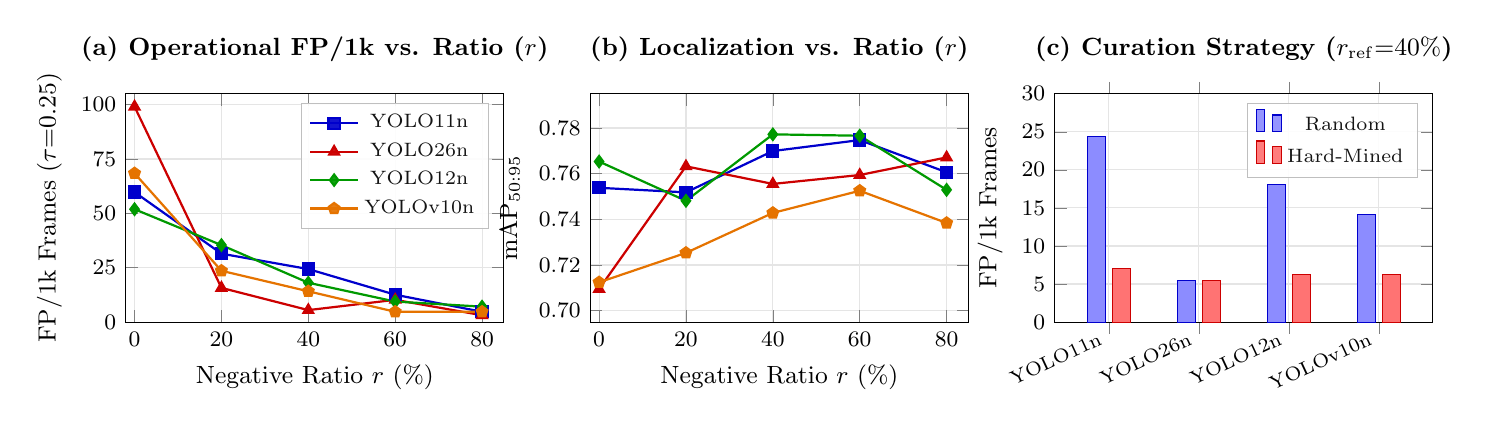
\begin{tikzpicture}
\begin{groupplot}[
group style={
group size=3 by 1,
horizontal sep=1.1cm
},
scale only axis,
width=4.8cm, height=2.9cm,
tick label style={font=\footnotesize},
label style={font=\small},
title style={font=\small\bfseries, yshift=2pt},
grid=major, grid style={gray!20}
]
% (a) FP/1k vs Ratio
\nextgroupplot[
title={(a) Operational FP/1k vs. Ratio ($r$)},
xlabel={Negative Ratio $r$ (\%)},
ylabel={FP/1k Frames ($\tau{=}0.25$)},
xmin=-2, xmax=85, ymin=0, ymax=105,
xtick={0,20,40,60,80},
ytick={0,25,50,75,100},
legend style={
at={(0.96,0.96)}, anchor=north east,
font=\scriptsize, fill=white, fill opacity=0.92,
draw=gray!50
}
]
\addplot[color=blue!80!black, mark=square*, thick] coordinates {(0,59.75) (20,31.45) (40,24.37) (60,12.58) (80,4.72)};
\addlegendentry{YOLO11n}
\addplot[color=red!80!black, mark=triangle*, thick] coordinates {(0,99.06) (20,15.72) (40,5.50) (60,10.22) (80,3.14)};
\addlegendentry{YOLO26n}
\addplot[color=green!60!black, mark=diamond*, thick] coordinates {(0,51.89) (20,35.38) (40,18.08) (60,9.43) (80,7.08)};
\addlegendentry{YOLO12n}
\addplot[color=orange!90!black, mark=pentagon*, thick] coordinates {(0,68.40) (20,23.58) (40,14.15) (60,4.72) (80,4.72)};
\addlegendentry{YOLOv10n}

% (b) mAP50:95 vs Ratio
\nextgroupplot[
title={(b) Localization vs. Ratio ($r$)},
xlabel={Negative Ratio $r$ (\%)},
ylabel={$\mathrm{mAP}_{50:95}$},
xmin=-2, xmax=85, ymin=0.695, ymax=0.795,
xtick={0,20,40,60,80},
ytick={0.70,0.72,0.74,0.76,0.78},
yticklabel style={
/pgf/number format/fixed,
/pgf/number format/precision=2,
/pgf/number format/zerofill
}
]
\addplot[color=blue!80!black, mark=square*, thick] coordinates {(0,0.7538) (20,0.7518) (40,0.7699) (60,0.7747) (80,0.7606)};
\addplot[color=red!80!black, mark=triangle*, thick] coordinates {(0,0.7095) (20,0.7632) (40,0.7555) (60,0.7594) (80,0.7671)};
\addplot[color=green!60!black, mark=diamond*, thick] coordinates {(0,0.7653) (20,0.7481) (40,0.7772) (60,0.7766) (80,0.7529)};
\addplot[color=orange!90!black, mark=pentagon*, thick] coordinates {(0,0.7124) (20,0.7253) (40,0.7428) (60,0.7525) (80,0.7384)};

% (c) Random vs Hard-Mined Bar Chart
\nextgroupplot[
title={(c) Curation Strategy ($r_{\mathrm{ref}}{=}40\%$)},
ybar=2.5pt, bar width=6.5pt,
enlarge x limits=0.20,
ylabel={FP/1k Frames},
symbolic x coords={YOLO11n, YOLO26n, YOLO12n, YOLOv10n},
xtick=data,
x tick label style={rotate=25, anchor=east, font=\scriptsize},
ymin=0, ymax=30,
ytick={0,5,10,15,20,25,30},
legend style={
at={(0.96,0.96)}, anchor=north east,
font=\scriptsize, fill=white, fill opacity=0.92,
draw=gray!50
}
]
\addplot[fill=blue!45, draw=blue!80!black] coordinates {(YOLO11n,24.37) (YOLO26n,5.50) (YOLO12n,18.08) (YOLOv10n,14.15)};
\addlegendentry{Random}
\addplot[fill=red!55, draw=red!80!black] coordinates {(YOLO11n,7.08) (YOLO26n,5.50) (YOLO12n,6.29) (YOLOv10n,6.29)};
\addlegendentry{Hard-Mined}
\end{groupplot}
\end{tikzpicture}
\caption{Cross-architecture empirical findings: (a) Operational false-alarm rates ($\mathrm{FP/1k}$) decrease monotonically in aggregate as negative ratio $r$ scales, converging to $3.14$--$7.08\,\mathrm{FP/1k}$ at $r{=}80\%$ (models in (a) and (b) share identical line/marker coding); (b) Bounding-box localization accuracy ($\mathrm{mAP}_{50:95}$) remains robust across negative dilution, confirming background suppression preserves learned foreground representations; (c) Hard-negative curation at matched cardinality ($r_{\mathrm{ref}}{=}40\%$, $N{=}4{,}001$) delivers substantial false-alarm reductions for attention and dual-head architectures while pure convolution hits an architectural saturation floor.}
\label{fig:empirical_summary}
\end{figure*}

\subsection{Hard-Negative Curation vs.\ Random Sampling (RQ2)}
\label{subsec:rq2_results}
Table~\ref{tab:rq2} benchmarks hard-negative mining against uniform random sampling
at the compute-efficient reference ratio $r_{\mathrm{ref}} = 40\%$, with strictly
matched cardinality ($N{=}4{,}001$ frames).

\begin{table}[t]
\caption{Hard-Negative Mining vs.\ Random Sampling at Matched Cardinality ($r_{\mathrm{ref}}{=}40\%$, RQ2)}
\label{tab:rq2}
\centering
\setlength{\tabcolsep}{4pt}
\begin{tabular}{llcccc}
\toprule
\textbf{Detector} & \textbf{Curation} & \textbf{$\mathrm{mAP}_{50}$} &
\textbf{$\mathrm{mAP}_{50:95}$} & \textbf{$\mathrm{FP/1k}$} &
\textbf{$\%\,\Delta$} \\
\midrule
\multirow{2}{*}{YOLO11n}
& Random     & 0.9932 & 0.7699 & 24.37 & \multirow{2}{*}{\textbf{-71.0\%}} \\
& Hard-Mined & \textbf{0.9946} & \textbf{0.7786} & \textbf{7.08} & \\
\midrule
\multirow{2}{*}{YOLO26n}
& Random     & 0.9830 & 0.7555 & \textbf{5.50} & \multirow{2}{*}{0.0\%} \\
& Hard-Mined & \textbf{0.9845} & \textbf{0.7585} & \textbf{5.50} & \\
\midrule
\multirow{2}{*}{YOLO12n}
& Random     & 0.9882 & 0.7772 & 18.08 & \multirow{2}{*}{\textbf{-65.2\%}} \\
& Hard-Mined & \textbf{0.9933} & \textbf{0.7838} & \textbf{6.29} & \\
\midrule
\multirow{2}{*}{YOLOv10n}
& Random     & 0.9615 & 0.7428 & 14.15 & \multirow{2}{*}{\textbf{-55.6\%}} \\
& Hard-Mined & \textbf{0.9836} & \textbf{0.7697} & \textbf{6.29} & \\
\bottomrule
\end{tabular}
\vspace{1pt}
{\footnotesize Evaluated on 1,272 negative test frames ($\tau{=}0.25$, matched $N{=}4{,}001$ training frames). $\%\,\Delta$: relative change in $\mathrm{FP/1k}$. Bold marks best condition per architecture. Dual-seed validation ($\text{seed}{=}42,43$) confirms cross-seed stability with $-52.6\%$ to $-67.8\%$ reductions across attention and dual-head models.}
\end{table}

The comparative results in Table~\ref{tab:rq2} and Fig.~\ref{fig:empirical_summary}c reveal a sharp architectural dichotomy in curation response.

\noindent\textbf{Curation Saturation in Pure Convolutions.}
For YOLO26n, hard-negative mining yields zero change in operational false alarms ($0.0\%$ reduction, remaining flat at $5.50\,\mathrm{FP/1k}$). Pure reparameterized convolutions saturate their background discriminative capacity once localized spatial filters learn dominant cabin textures; localized $3 \times 3$ receptive fields lack the global context to resolve rare macro-level interior structures. Consequently, substituting random negatives with mined negatives supplies redundant local gradient signals, offering no marginal benefit.

\noindent\textbf{Amplified Gains in Attention and Dual-Assignment Models.}
In stark contrast, models equipped with attention (YOLO11n, YOLO12n) and dual-assignment heads (YOLOv10n) achieve dramatic false-alarm reductions ($55.6\%$--$71.0\%$) alongside concurrent gains in localization accuracy ($\mathrm{mAP}_{50:95}$ increasing by up to $+0.027$). Attention layers possess flexible, global hypothesis spaces. Uniform random sampling predominantly selects low-entropy background patches (plain headrests, uniform window glass) that offer negligible gradient feedback to global query-key projection weights. High-entropy hard negatives capture complex ambient reflections and driver silhouettes that provoke spurious cross-attention activations, forcing attention layers to decorrelate non-target contextual patterns from true driver cues. For YOLOv10n, mined negatives penalize spurious multi-anchor activations in the auxiliary head, sharpening the decision boundary of the one-to-one inference branch.

\noindent\textbf{The Curation Rule: Curate for Attention, Sample for Convolutions.}
These results demonstrate that curation efficacy is governed by the detector's architectural receptive field. Edge engineering teams deploying pure convolutional backbones can safely bypass multi-stage mining pipelines, relying on simple random background sampling. Conversely, teams deploying attention or dual-assignment architectures should prioritize hard-negative curation, unlocking major reliability gains at matched dataset cardinality.

\subsection{Operational Deployment Cost Translation}
\label{subsec:cost_results}
Table~\ref{tab:deployment} translates empirical $\mathrm{FP/1k}$ values into estimated hourly nuisance alert rates ($\mathcal{A}_h$) via~\eqref{eq:nuisance} across three standard camera streaming frequencies.

\begin{table}[t]
\caption{Projected Nuisance Alerts per Hour ($\mathcal{A}_h$) Across Frame Rates}
\label{tab:deployment}
\centering
\setlength{\tabcolsep}{5pt}
\begin{tabular}{llccc}
\toprule
\textbf{Detector} & \textbf{Training Split} & \textbf{5\,FPS} &
\textbf{15\,FPS} & \textbf{30\,FPS} \\
\midrule
\multirow{2}{*}{YOLO11n}
& 0\% Neg.\ Baseline       & 870   & 2{,}610 & 5{,}220 \\
& 80\% Neg.\ Ratio         & 69    & 206     & 412     \\
\midrule
\multirow{2}{*}{YOLO26n}
& 0\% Neg.\ Baseline       & 1{,}443 & 4{,}328 & 8{,}655 \\
& 80\% Neg.\ Ratio         & \textbf{46} & \textbf{137} & \textbf{274} \\
\midrule
\multirow{2}{*}{YOLO12n}
& 0\% Neg.\ Baseline       & 756   & 2{,}267 & 4{,}534 \\
& 80\% Neg.\ Ratio         & 103   & 309     & 619     \\
\midrule
\multirow{2}{*}{YOLOv10n}
& 0\% Neg.\ Baseline       & 996   & 2{,}989 & 5{,}977 \\
& 80\% Neg.\ Ratio         & 69    & 206     & 412     \\
\bottomrule
\end{tabular}
\vspace{1pt}
{\footnotesize Modeled via~\eqref{eq:nuisance} using operational negative prevalence $p_{\mathrm{neg}}{=}0.809$. Bold marks lowest alert rates.}
\end{table}

This translation formalizes a foundational principle in edge AIoT systems engineering: \textbf{inference latency is architecture-bound, whereas operational reliability is curation-bound.}

While all four models execute within real-time budgets ($7.7$--$21.7$\,ms, Table~\ref{tab:architectures}), operational usability is dictated by training-data composition. An ultra-fast detector running at $129$\,FPS is practically unusable if it generates thousands of false alarms per hour. As Table~\ref{tab:deployment} illustrates, baseline models trigger up to 8{,}655 nuisance alerts per hour at 30\,FPS. Scaling negative frames to 80\% slashes alert rates by up to 94.7\% without altering a single parameter or instruction. In continuous edge AIoT, data curation is the definitive lever for operational uptime.

\section{Discussion}
\label{sec:discussion}

\subsection{Practical Guidelines for AIoT Data Curation}
Our empirical findings offer two operational recommendations:

\noindent\textbf{1) False-Alarm Minimization (Safety-Critical AIoT):} For systems where false alarms degrade user trust or incur uplink costs, training at the 80\% negative ratio is globally superior across all four architectures. YOLO26n achieves the lowest false-alarm rate ($3.14\,\mathrm{FP/1k}$, yielding 46 alerts/hr at 5\,FPS), making pure reparameterized convolutions well-suited for high-precision, low-power sensing.

\noindent\textbf{2) Compute-Constrained Training and High Localization:} When training budgets limit dataset size, a 40\% negative ratio offers the best trade-off. It retains $\ge 98.3\%$ of peak $\mathrm{mAP}_{50}$, achieves top-tier localization ($\mathrm{mAP}_{50:95} = 0.7772$ for YOLO12n), and captures the bulk of false-alarm suppression with less than one-third the negative volume of the 80\% split.

Furthermore, while detection sensitivity ($\mathrm{mAP}_{50}$) exhibits broad stability across ratios ($r \in [40\%, 80\%]$), false-positive suppression magnitudes diverge sharply: YOLO26n suppresses false alarms by $31.5\times$, YOLOv10n by $14.5\times$, YOLO11n by $12.7\times$, and YOLO12n by $7.3\times$. This divergence confirms that edge architects cannot decouple data curation from detector selection: models relying on attention mechanisms require higher negative densities to achieve comparable background suppression as pure convolutional backbones.

\subsection{Limitations}
Several methodological constraints contextualize our findings:
\begin{itemize}\setlength{\itemsep}{0pt}\setlength{\parskip}{0pt}\setlength{\parsep}{0pt}
\item \textbf{Training Step Confound:} Fixed 100-epoch training across variable dataset sizes (2,401 to 12,005 frames) affords the 80\% condition more gradient steps; step-ablations remain future work.
\item \textbf{Mining Purity Variations:} Candidate pools contained differing fractions of mined false alarms (34.2\%--59.2\%) due to deterministic backfill to $N{=}1{,}600$.
\item \textbf{Frame-Level Partitioning:} Consecutive frames share vehicle cabins and lighting; near-ceiling detection ($\mathrm{mAP}_{50} > 0.97$) may partly reflect temporal correlation rather than cross-vehicle generalization.
\item \textbf{Foreground Class Imbalance:} The positive core is dominated by \texttt{phone\_use} (81.2\%), so aggregate mAP primarily tracks majority-class accuracy.
\item \textbf{Multi-Seed Replication \& Stability:} Dual-seed replication ($\text{seed}{=}42, 43$) across all four architectures confirms consistent dynamics across both questions: non-zero RQ1 splits show tight variance ($\pm 0.56$ to $\pm 5.56\,\mathrm{FP/1k}$), while RQ2 curation consistently slashes false alarms by $52.6\%$--$67.8\%$ for attention and dual-head models, with near-floor stability ($6.29$--$7.08\,\mathrm{FP/1k}$; $\pm 0.00$ for YOLO11n and YOLO12n).
\end{itemize}

\section{Conclusion}
\label{sec:conclusion}
This paper investigated the interaction between negative-frame training curation and edge detector architectures across matched-capacity ($2.3$--$2.6$\,M parameter) models in continuous AIoT sensing. While models exhibit diverse suppression trajectories across negative ratios, all four architectures converge to a narrow false-positive band ($3.14$--$7.08\,\mathrm{FP/1k}$) under high negative prevalence ($r{=}80\%$). Because on-device latency remains strictly architecture-bound ($7.7$--$21.7$\,ms), operational nuisance alert rates are primarily governed by training-data composition rather than architectural choice. Edge AIoT practitioners should curate negative frames to reflect operational background dominance first, selecting detector backbones based on hardware latency targets rather than relying on architectural inductive biases alone to suppress false alarms.

\section*{Acknowledgment}
Acknowledgment omitted for double-blind review.

\begin{thebibliography}{00}
\setlength{\itemsep}{0.6pt}
\setlength{\parskip}{0pt}
\bibitem{b1}
T.-Y. Lin, P. Goyal, R. Girshick, K. He, and P. Doll\'{a}r,
``Focal loss for dense object detection,''
in \textit{Proc. IEEE/CVF Int. Conf. Comput. Vision (ICCV)}, Oct. 2017, pp. 2980--2988.
\bibitem{b2}
X. Wang, X. Hu, C. Chen, Z. Fan, and S. Peng,
``Improving object detection with consistent negative sample mining,''
in \textit{Proc. Int. Conf. Neural Inf. Process. (ICONIP)}, LNCS vol. 11954, Springer, 2019, pp. 248--259.
\bibitem{b3}
S. Zhang, C. Chi, Y. Yao, Z. Lei, and S. Li,
``Bridging the gap between anchor-based and anchor-free detection via adaptive training sample selection,''
in \textit{Proc. IEEE/CVF Conf. Comput. Vis. Pattern Recognit. (CVPR)}, Jun. 2020, pp. 9759--9768.
\bibitem{b4}
B. Singh, M. Najibi, and L. S. Davis,
``SNIPER: Efficient multi-scale training,''
in \textit{Proc. Adv. Neural Inf. Process. Syst. (NeurIPS)}, vol. 31, Dec. 2018, pp. 9333--9343.
\bibitem{b5}
S. Beery, G. Van Horn, and P. Perona,
``Recognition in Terra Incognita,''
in \textit{Proc. Eur. Conf. Comput. Vision (ECCV)}, Sep. 2018, pp. 456--473.
\bibitem{b6}
P. F. Felzenszwalb, R. B. Girshick, D. McAllester, and D. Ramanan,
``Object detection with discriminatively trained part-based models,''
\textit{IEEE Trans. Pattern Anal. Mach. Intell.}, vol. 32, no. 9, pp. 1627--1645, Sep. 2010.
\bibitem{b7}
T. Gupta, A. Schwing, and D. Hoiem,
``No-frills human-object interaction detection,''
in \textit{Proc. IEEE/CVF Int. Conf. Comput. Vision (ICCV)}, Oct. 2019, pp. 1960--1969.
\bibitem{b8}
Ultralytics,
``Tips for best training results: Background images,''
\textit{Ultralytics Documentation}, 2024. [Online]. Available: \url{https://docs.ultralytics.com/guides/model-training-tips/}
\bibitem{b9}
G. Jocher and J. Qiu,
``Ultralytics YOLO11,''
\textit{GitHub repository}, 2024. [Online]. Available: \url{https://github.com/ultralytics/ultralytics}
\bibitem{b10}
Ultralytics,
``Ultralytics YOLO26 architecture and models,''
\textit{Ultralytics Documentation and Repository}, 2026. [Online]. Available: \url{https://docs.ultralytics.com/models/yolo26/}
\bibitem{b11}
Y. Tian, Q. Ye, and M. Doermann,
``YOLOv12: Attention-centric real-time object detectors,''
\textit{arXiv preprint arXiv:2502.12524}, Feb. 2025.
\bibitem{b12}
A. Sengupta, V. Sharma, and R. Mall,
``Computer vision for in-cabin driver monitoring: A comprehensive review,''
\textit{IEEE Trans. Intell. Transp. Syst.}, vol. 24, no. 9, pp. 8945--8965, Sep. 2023.
\bibitem{b13}
J. Chen, K. Li, Z. Rong, and K. Bilgic,
``False alert suppression and energy-efficient edge inferencing in smart surveillance IoT,''
\textit{IEEE Internet Things J.}, vol. 10, no. 14, pp. 12340--12352, Jul. 2023.
\bibitem{b14}
A. Shrivastava, A. Gupta, and R. Girshick,
``Training region-based object detectors with online hard example mining,''
in \textit{Proc. IEEE Conf. Comput. Vis. Pattern Recognit. (CVPR)}, Jun. 2016, pp. 761--769.
\bibitem{b15}
E. Wang, M. Davis, S. Xu, and T. Huang,
``Deep learning on micro-edge devices: A survey on architectural efficiency and inference constraints,''
\textit{IEEE Access}, vol. 11, pp. 45120--45138, May 2023.
\bibitem{b16}
X. Li \textit{et al.},
``Generalized focal loss: Learning qualified and distributed bounding boxes for dense object detection,''
in \textit{Proc. Adv. Neural Inf. Process. Syst. (NeurIPS)}, vol. 33, Dec. 2020, pp. 18312--18323.
\bibitem{b17}
L. Fridman, P. Toyman, and B. Seaman,
``Cognitive load and distraction detection via multi-sensor driver monitoring in automated vehicles,''
\textit{IEEE Trans. Intell. Veh.}, vol. 4, no. 2, pp. 270--281, Jun. 2019.
\bibitem{b18}
State Farm,
``State Farm Distracted Driver Detection,''
\textit{Kaggle Competition Dataset}, 2016. [Online]. Available: \url{https://www.kaggle.com/c/state-farm-distracted-driver-detection}
\bibitem{b19}
I. Ortega \textit{et al.},
``DMD: A large-scale multi-modal driver monitoring dataset for attention and distraction analysis,''
in \textit{Proc. IEEE/CVF Conf. Comput. Vis. Pattern Recognit. Workshops (CVPRW)}, Jun. 2020, pp. 498--507.
\bibitem{b20}
A. Wang \textit{et al.},
``YOLOv10: Real-time end-to-end object detection,''
\textit{arXiv preprint arXiv:2405.14458}, May 2024.
\end{thebibliography}

\end{document}

